\chapter{PRELIMINARY RESULTS AND DISCUSSION}
\label{chap:results}

This chapter details the preliminary findings derived from the implementation of the proposed 2.5D terrain-aware path planning framework. By systematically evaluating the planner across multiple synthetic agricultural topographies, this analysis seeks to quantify the impacts of the terrain-aware Step Traversal Cost (STC) and the subsequent B-spline refinement. The preliminary results presented herein serve to validate the foundational hypotheses of this research and demonstrate the planner's capability to generate feasible, safe, and efficient trajectories over uneven agricultural terrain.

\section{Cross-Map Trajectory Layouts}
Figure \ref{fig:cross_map_trajectory_layouts} presents the route overlays obtained under the Slope Cost Weight (SCW) sweep for all three terrain profiles. This qualitative result highlights how the proposed path planning framework redistributes the path corridor as terrain relief increases. In the low-gradient map, the trajectories remain tightly clustered, indicating that multiple SCW settings still favor nearly the same broad corridor due to the uniform topography. In the medium-relief map, the separation between overlays becomes more pronounced, particularly in regions where the planner can actively trade directness for flatter traversal. Crucially, in the high-relief map, the route family spreads most strongly, demonstrating that high SCW values successfully force substantial and necessary detours around steep, potentially hazardous terrain features.

\begin{figure*}[htbp]
\centering
\IfFileExists{figures/map1_flat_route_overlay.pdf}{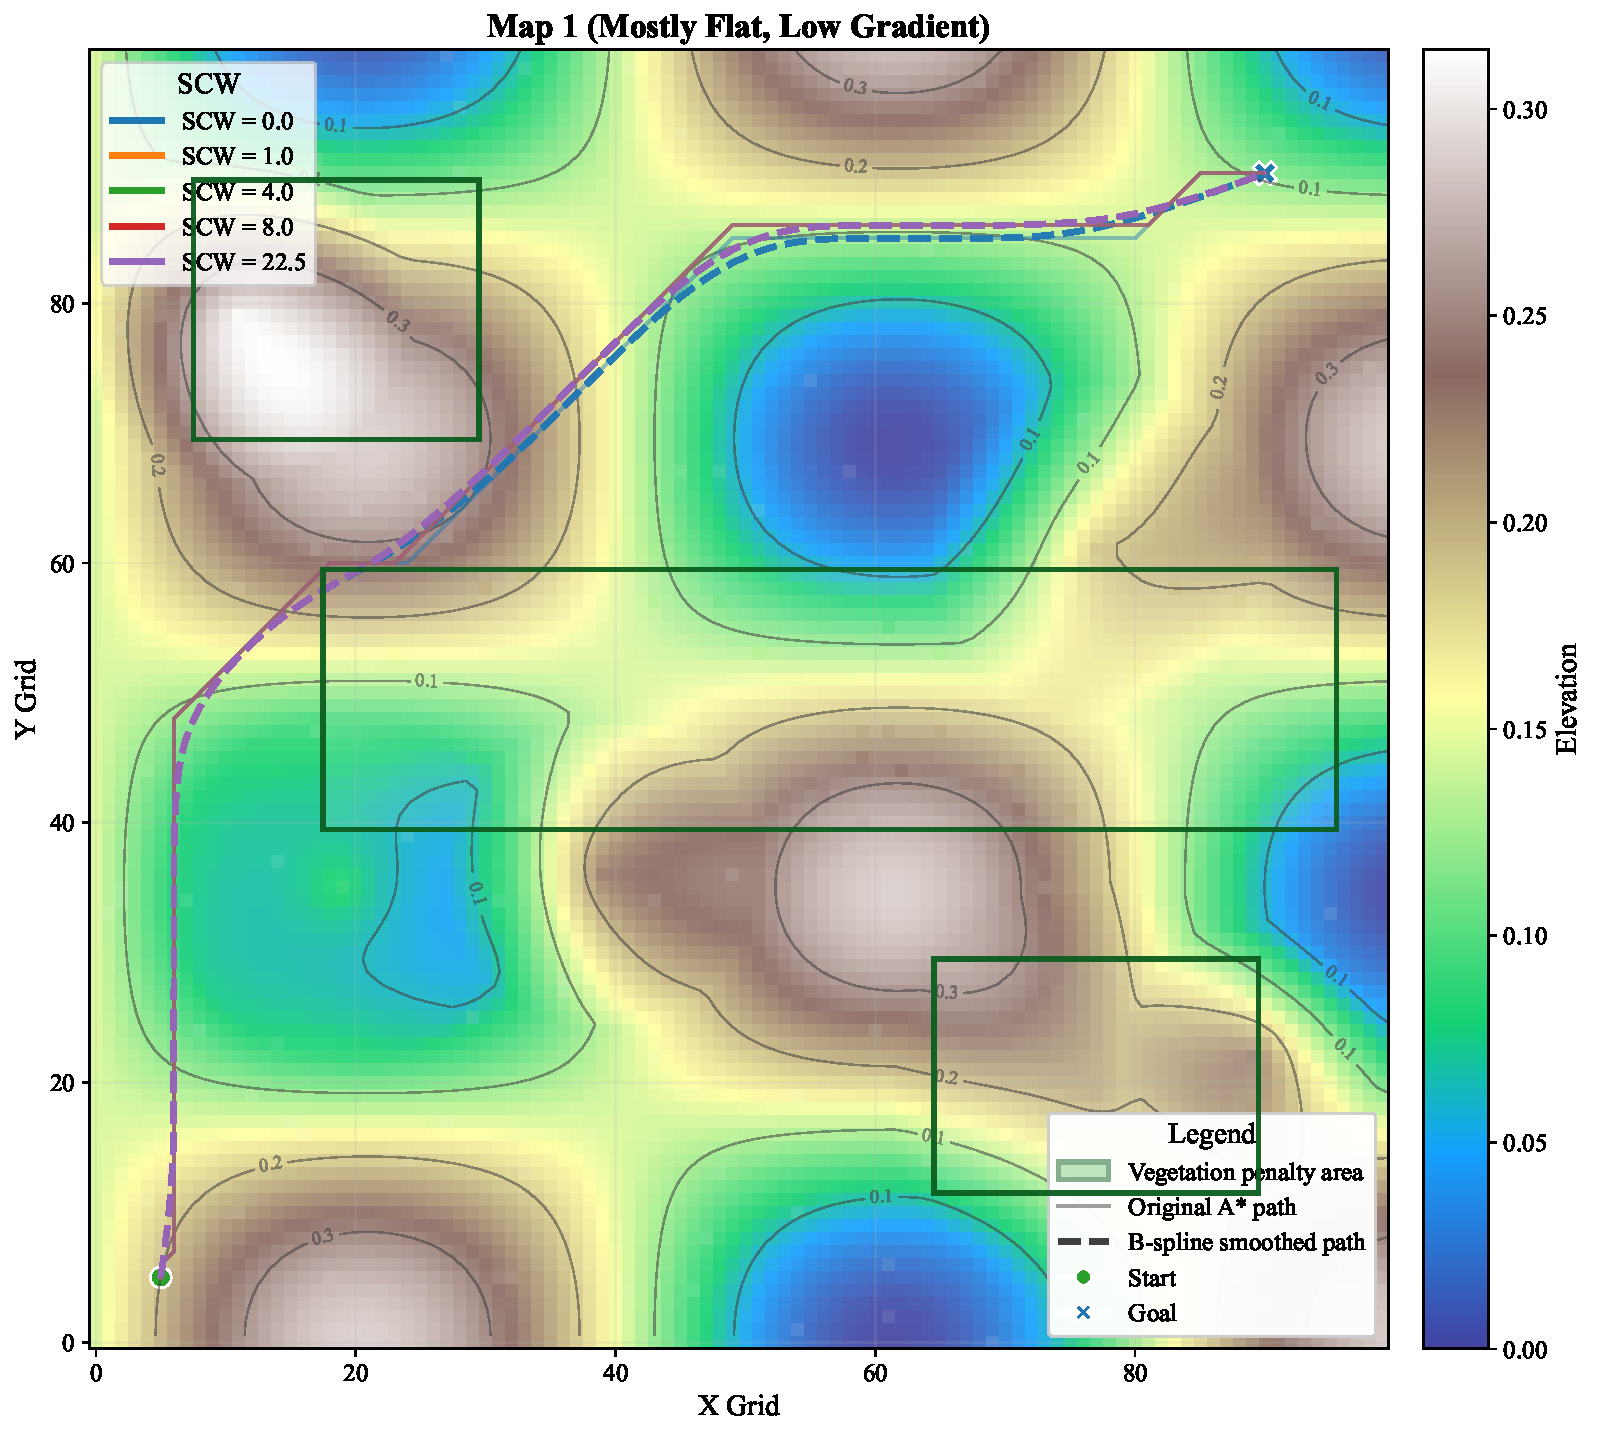
\includegraphics[width=0.48\textwidth]{figures/map1_flat_route_overlay.pdf}}{\fbox{\parbox{0.46\textwidth}{\centering Missing map 1 trajectory layout}}}
\hfill
\IfFileExists{figures/map2_medium_route_overlay.pdf}{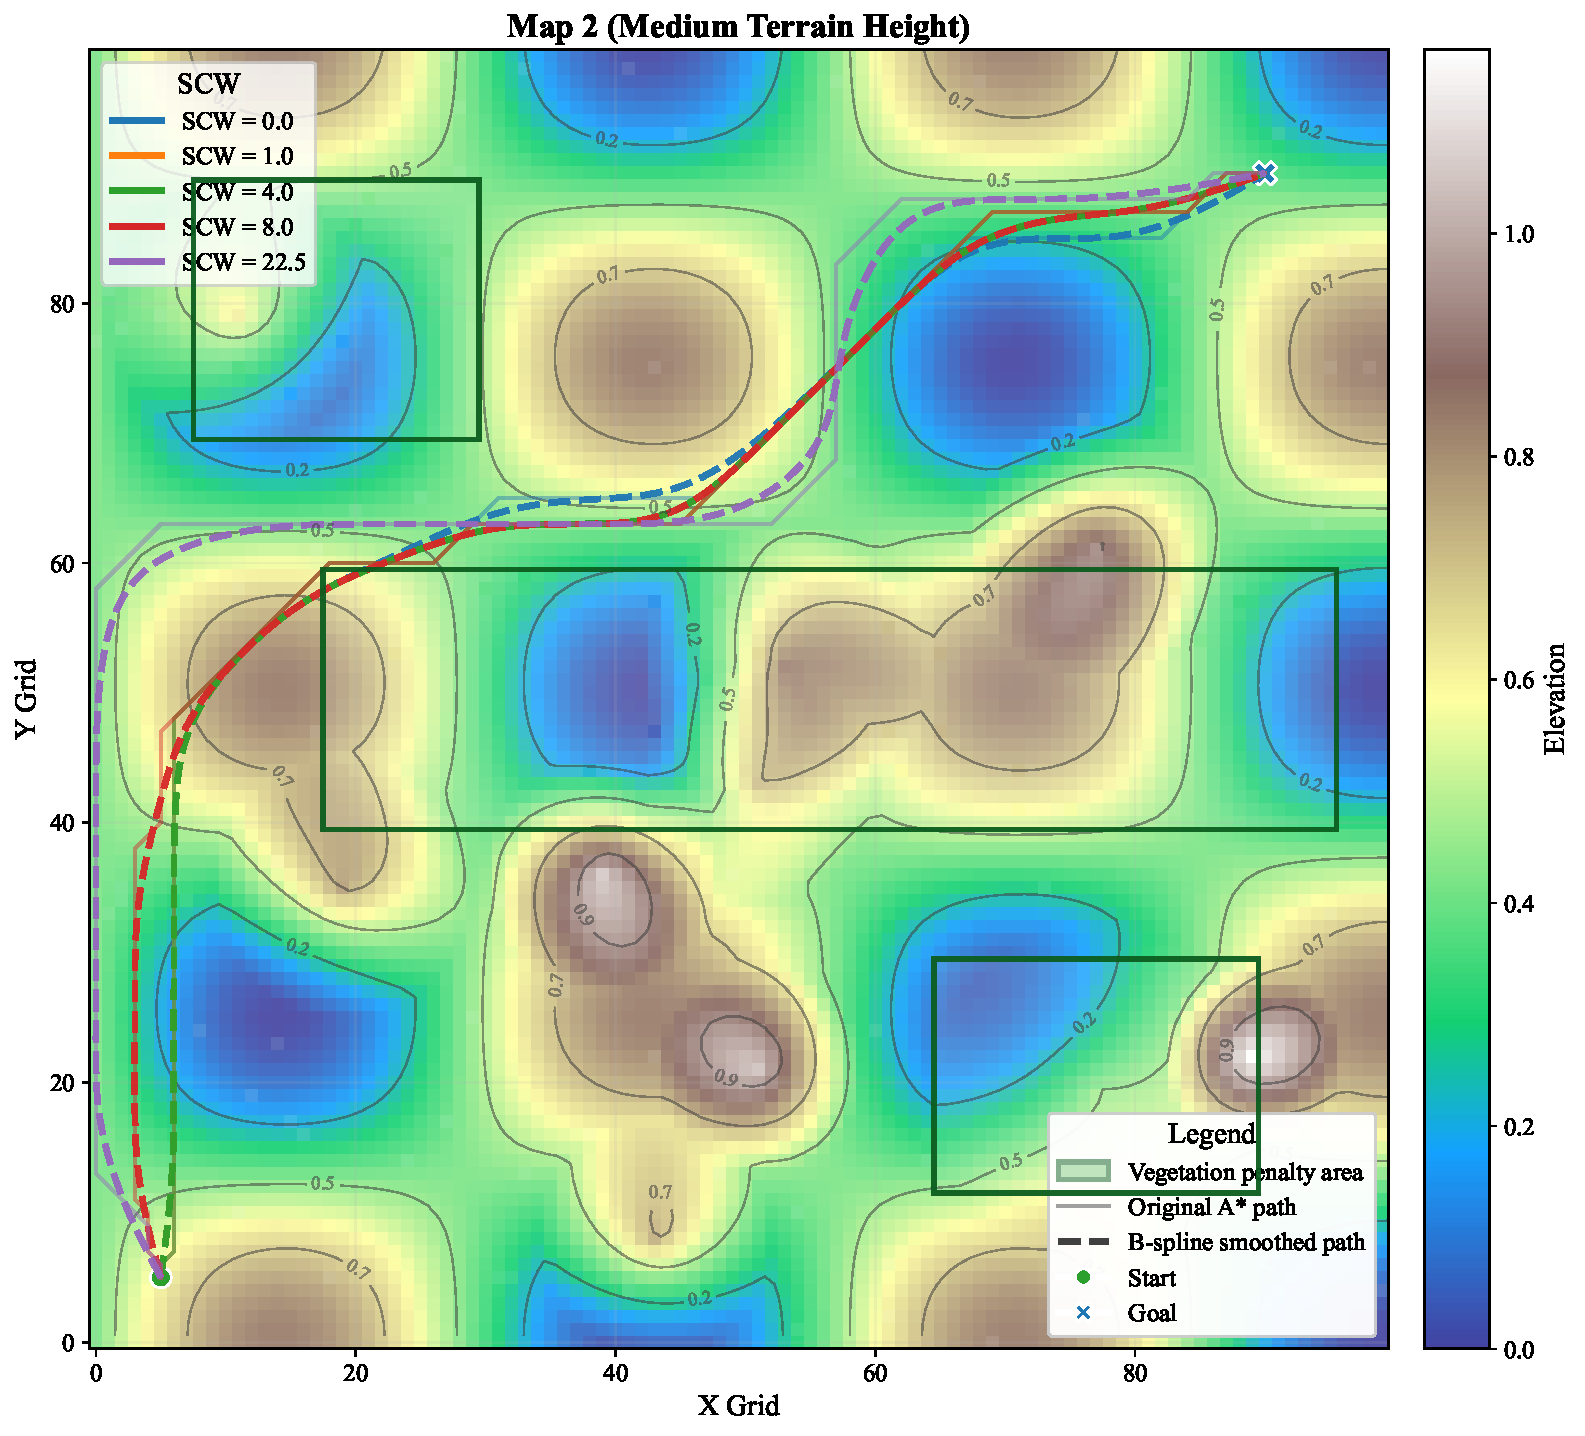
\includegraphics[width=0.48\textwidth]{figures/map2_medium_route_overlay.pdf}}{\fbox{\parbox{0.46\textwidth}{\centering Missing map 2 trajectory layout}}}

\vspace{0.6em}
\IfFileExists{figures/map3_high_route_overlay.pdf}{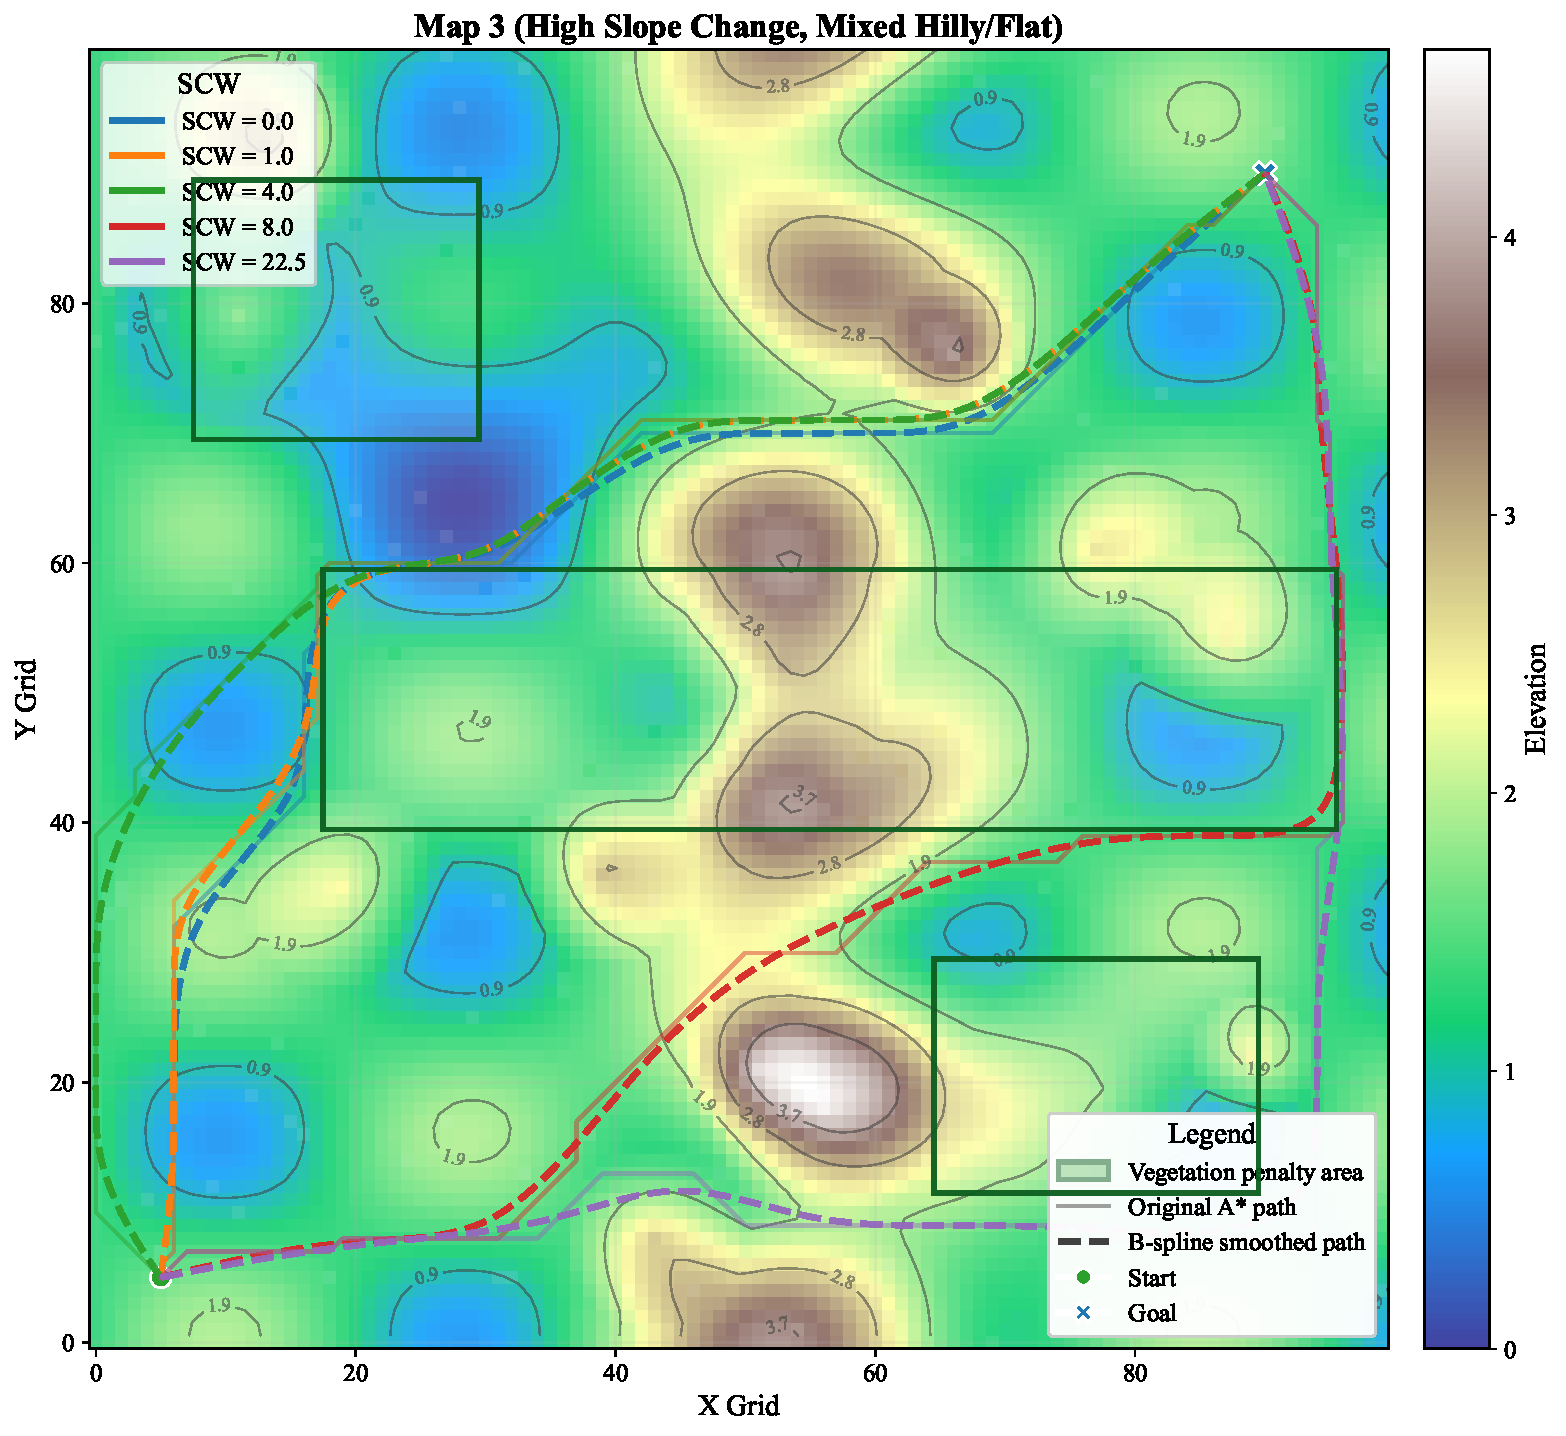
\includegraphics[width=0.62\textwidth]{figures/map3_high_route_overlay.pdf}}{\fbox{\parbox{0.60\textwidth}{\centering Missing map 3 trajectory layout}}}
\caption{Cross-map trajectory layouts under SCW variation. From left to right, the overlays correspond to low-gradient, medium-relief, and high-relief terrain. Terrain color shading, contour labels, and the elevation color bar expose the underlying height variation, while the increasing separation of trajectories demonstrates that terrain severity amplifies the rerouting effect of the slope-aware cost design.}
\label{fig:cross_map_trajectory_layouts}
\end{figure*}

The trajectory layouts provide the geometric interpretation for the quantitative trends reported in the subsequent analysis. Specifically, the increasing divergence of the route overlays explains why the high-relief terrain produces the strongest growth in path length, Energy Consumption Proxy (ECP), and Travel-Time Proxy (TTP) as the slope weight increases.

\section{Cross-Map Sensitivity to Slope Cost Weight}
Figure \ref{fig:cross_map_metric_trends} illustrates the metric response to SCW across the three distinct terrain profiles. The identical parameter sweep yields clearly different routing behaviors depending on terrain severity. In the low-gradient map, increasing SCW causes only moderate changes in path length, ECP, and TTP because the terrain inherently provides broad, low-cost corridors. The medium-relief map exhibits a stronger response, displaying visible growth in all three metrics as the planner increasingly prioritizes slope avoidance over spatial directness. The high-relief map manifests the largest sensitivity, confirming the premise that rugged agricultural terrain substantially amplifies the cost of conservative, slope-aware routing.

\begin{figure*}[htbp]
\centering
\IfFileExists{figures/map1_flat_metric_trends.pdf}{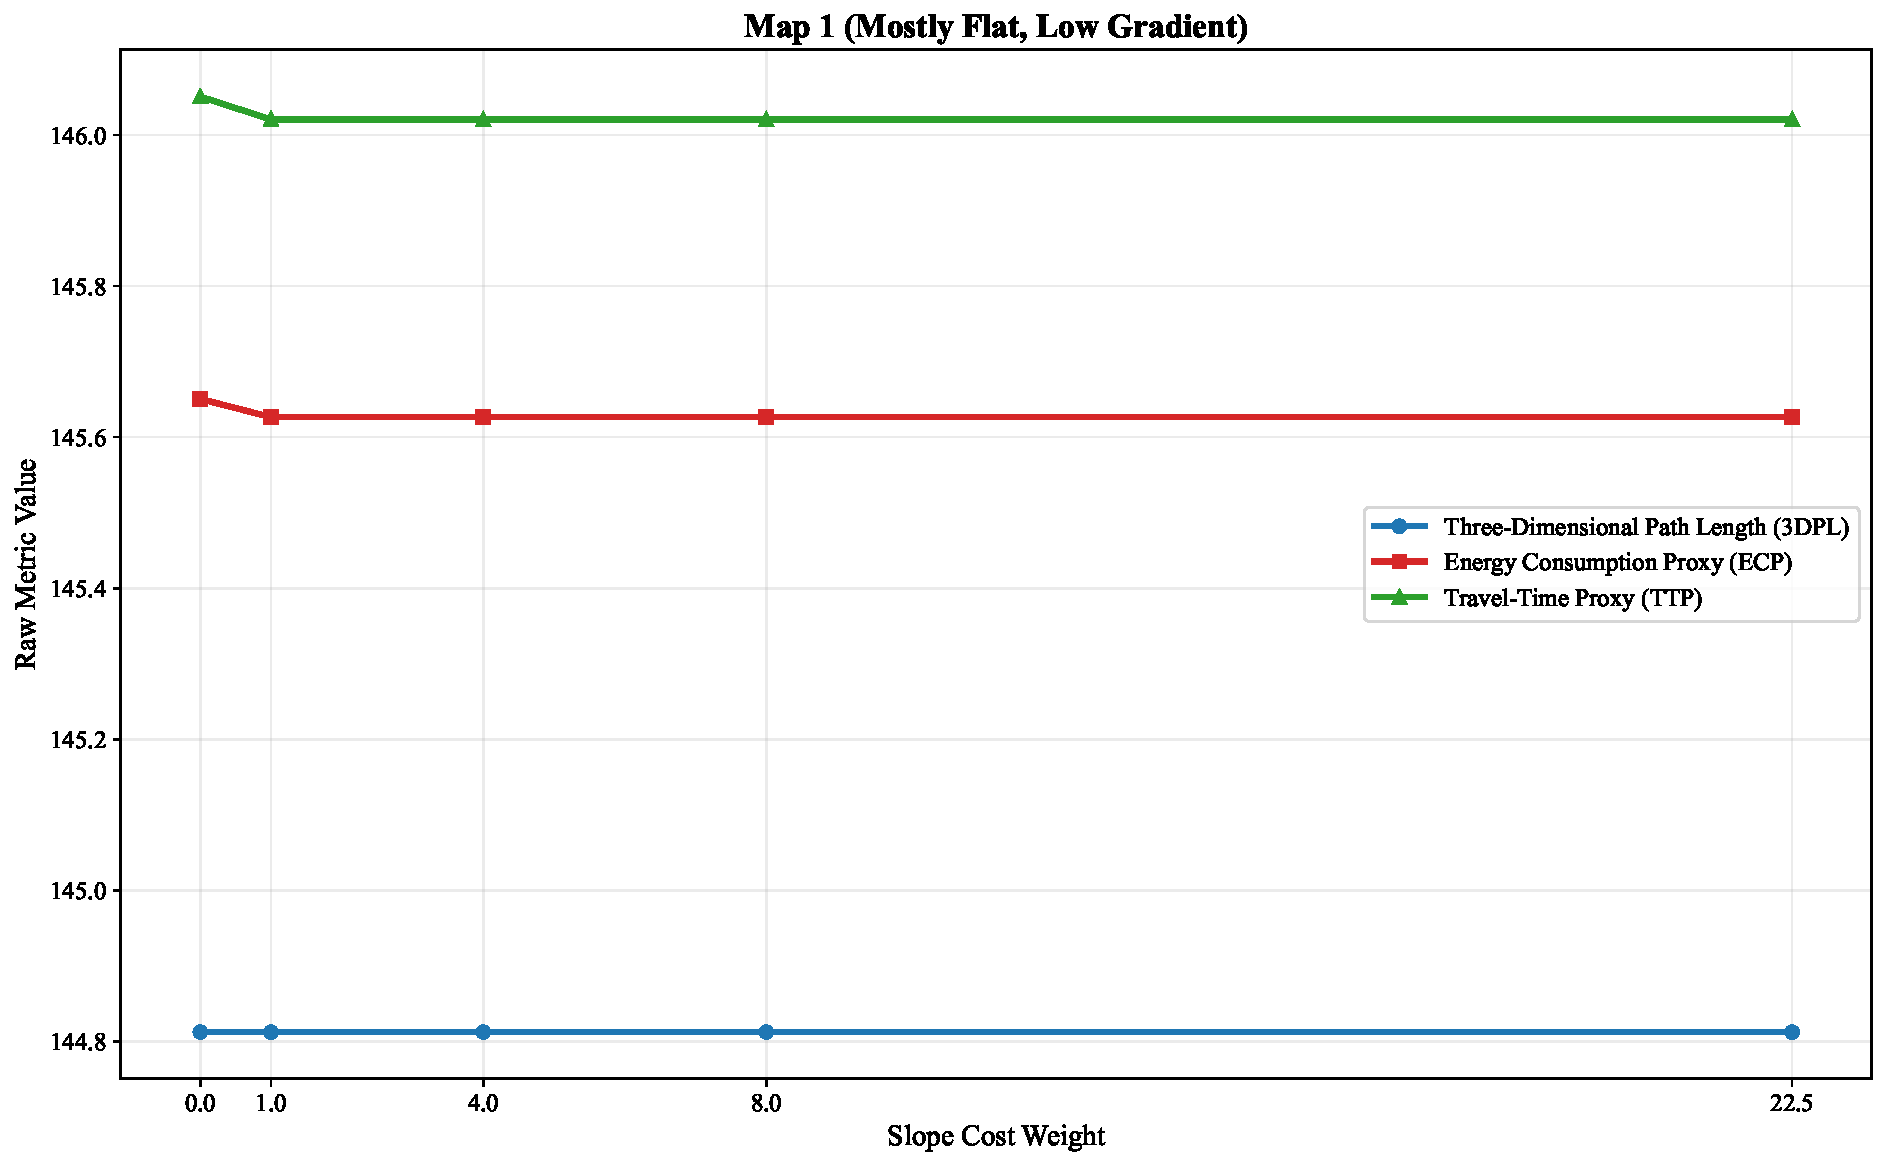
\includegraphics[width=0.48\textwidth]{figures/map1_flat_metric_trends.pdf}}{\fbox{\parbox{0.46\textwidth}{\centering Missing map 1 metric figure}}}
\hfill
\IfFileExists{figures/map2_medium_metric_trends.pdf}{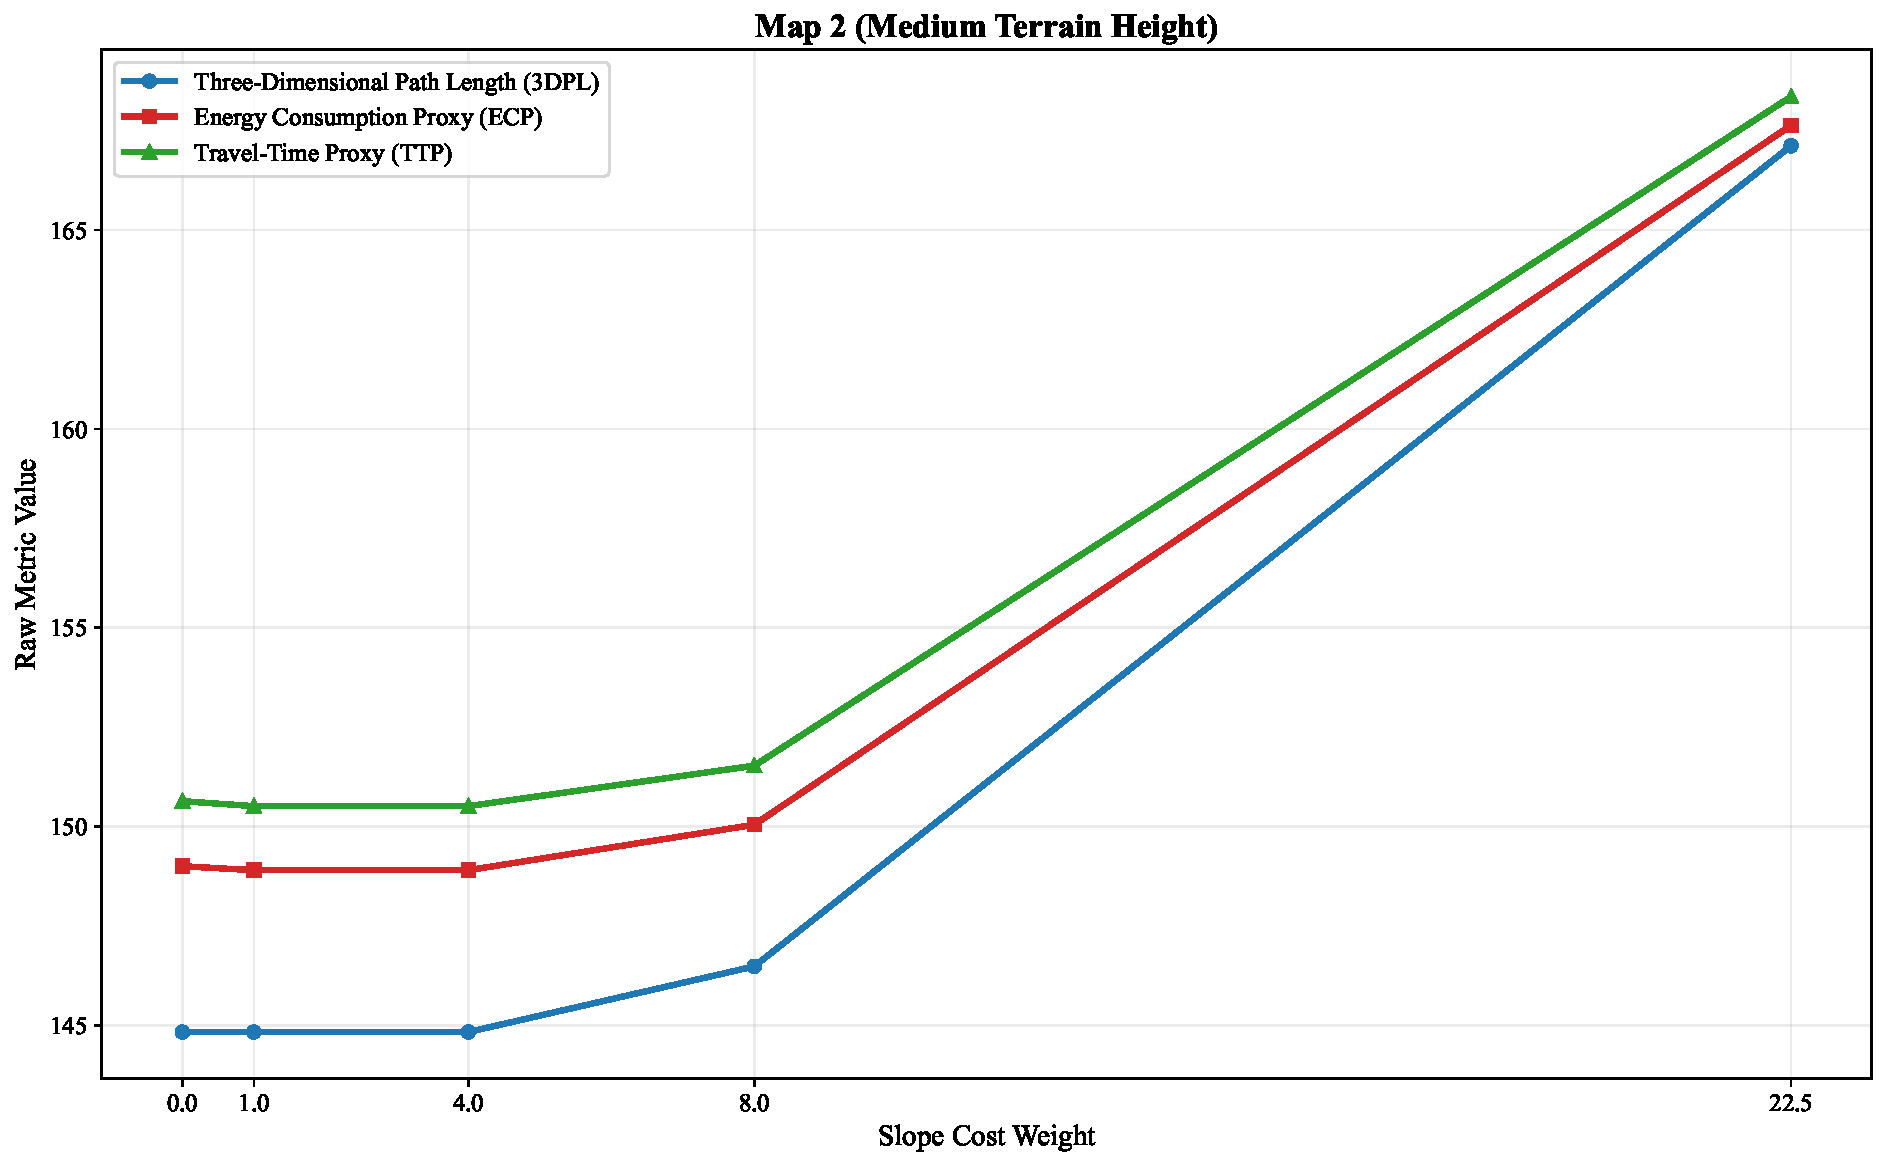
\includegraphics[width=0.48\textwidth]{figures/map2_medium_metric_trends.pdf}}{\fbox{\parbox{0.46\textwidth}{\centering Missing map 2 metric figure}}}

\vspace{0.6em}
\IfFileExists{figures/map3_high_metric_trends.pdf}{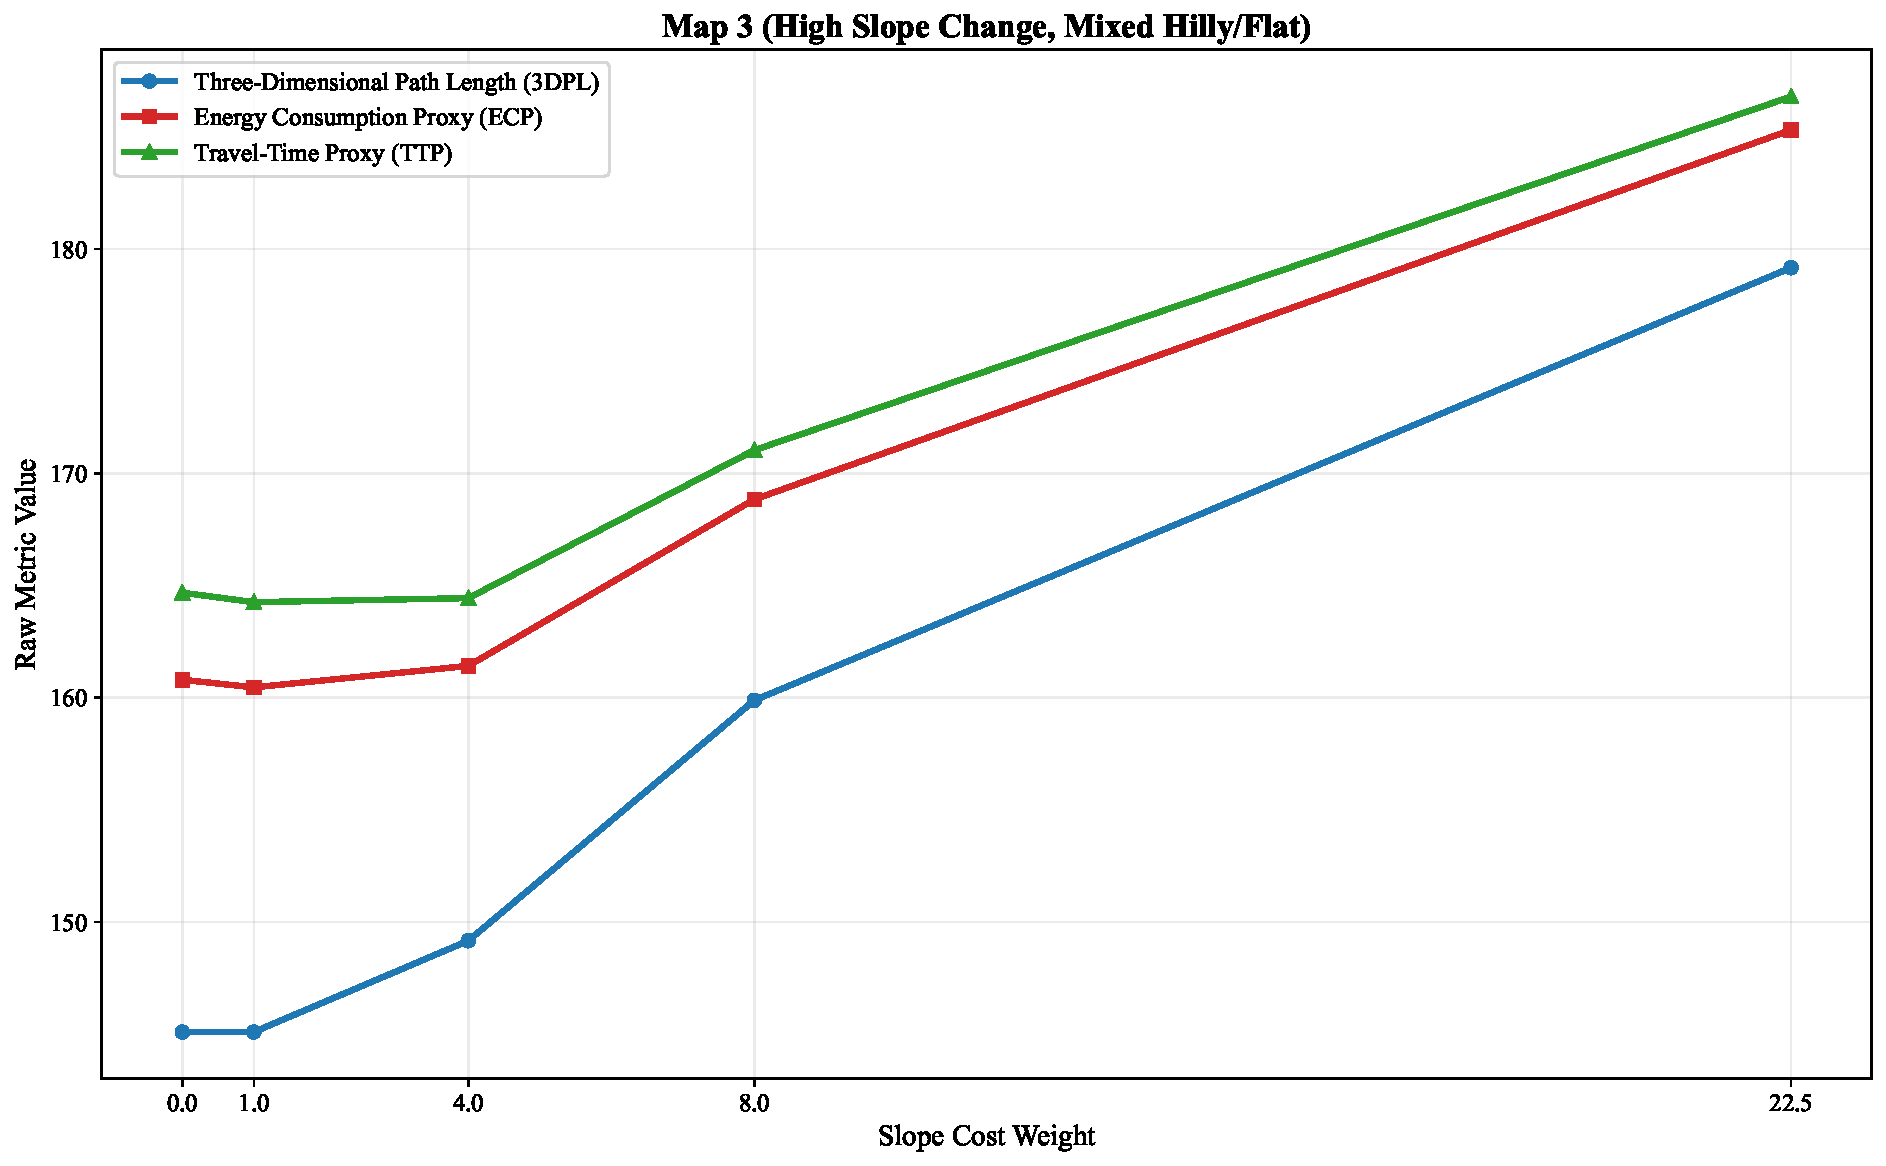
\includegraphics[width=0.62\textwidth]{figures/map3_high_metric_trends.pdf}}{\fbox{\parbox{0.60\textwidth}{\centering Missing map 3 metric figure}}}
\caption{Cross-map metric trends under SCW variation for low-gradient, medium-relief, and high-relief terrain. The separation between curves increases with terrain severity, indicating a stronger sensitivity of route quality to the slope-aware STC formulation.}
\label{fig:cross_map_metric_trends}
\end{figure*}

This cross-map behavior aligns seamlessly with the theoretical assertion that SCW does not act as a universal penalty with a uniform effect. Rather, it dynamically modulates the trade-off between route efficiency and slope avoidance in a highly terrain-dependent manner. In mild terrain, the planner successfully preserves relatively direct routes even at higher SCW values. Conversely, in rugged terrain, an identical increase in SCW enforces larger detours, consequentially inducing larger increases in both energy expenditure and travel time.

\section{Aggregate Multi-Pair Validation}
To rigorously evaluate whether the observed behavior is robust and independent of a specific start-goal coordinate selection, the experiment was repeated across three distinct start-goal pairs on each of the synthetic maps. Table \ref{tab:multi_pair_summary} reports the aggregate outcome averaged over 15 runs per map. The summary indicates average planning times ranging from 36.72 to 42.29 ms per run, and average B-spline smoothing plus validation times ranging from 12.44 to 12.47 ms. These timings remain computationally marginal relative to the primary search phase, reinforcing the practical real-time viability of the proposed post-processing pipeline at the specified grid resolution.

\begin{table*}[htbp]
\centering
\caption{Aggregate multi-pair summary across three start-goal pairs per map. Negative percentage changes indicate that the B-spline refinement algorithm successfully reduces the corresponding metric relative to the original A* path.}
\label{tab:multi_pair_summary}
\small
\begin{tabular}{lrrrrrrrr}
\toprule
Map & Runs & Plan (ms) & Smooth (ms) & $\Delta L$ (\%) & $\Delta T$ (\%) & $\Delta \theta$ (\%) & Veg. Samp. & Slope Viol. \\ 
\midrule
Map 1 & 15 & 36.72 & 12.44 & -5.22 & -5.21 & -88.59 & 41.3 & 0 \\ 
Map 2 & 15 & 38.94 & 12.47 & -5.06 & -4.98 & -87.98 & 29.9 & 0 \\ 
Map 3 & 15 & 42.29 & 12.46 & -6.28 & -5.40 & -89.03 & 39.5 & 0 \\ 
\bottomrule
\end{tabular}
\end{table*}

The aggregate metrics demonstrate that the B-spline refinement layer consistently improves global route smoothness without violating the localized sampled slope constraint. Across all three tested terrain profiles, the smoothed trajectory reduces the total spatial length by 5.06--6.28\%, reduces the travel-time proxy by 4.98--5.40\%, and substantially mitigates the mean turn angle by 87.98--89.03\%. The zero slope-violation count reported for all maps conclusively indicates that the sampled refined trajectories remain strictly feasible under the tested structural climbability threshold. While vegetation-exposure counts are nonzero, they remain definitively bounded and terrain-dependent, reflecting the fundamental principle that the smoothing operation preserves the qualitative safe corridor selected by the planner, rather than introducing unconstrained, destructive shortcuts through penalized regions.

\section{Quantitative Effect of B-Spline Refinement}
Figure \ref{fig:cross_map_bspline_metrics} visualizes the comparative metric analysis between the original discrete A* polyline and the refined continuous B-spline path for all three terrain profiles. The most pronounced and critical effect is the massive reduction in the mean turn angle, which conclusively confirms that the post-processing stage acts effectively as a geometric regularizer, eliminating sharp, kinematically infeasible corners. In the context of this preliminary evaluation, that fundamental geometric improvement is concurrently accompanied by moderate, yet consistent, reductions in total path length and time proxy, suggesting that the piecewise-linear A* path natively contains avoidable directional discontinuities that are efficiently smoothed without compromising sampled feasibility.

\begin{figure*}[htbp]
\centering
\IfFileExists{figures/map1_flat_bspline.pdf}{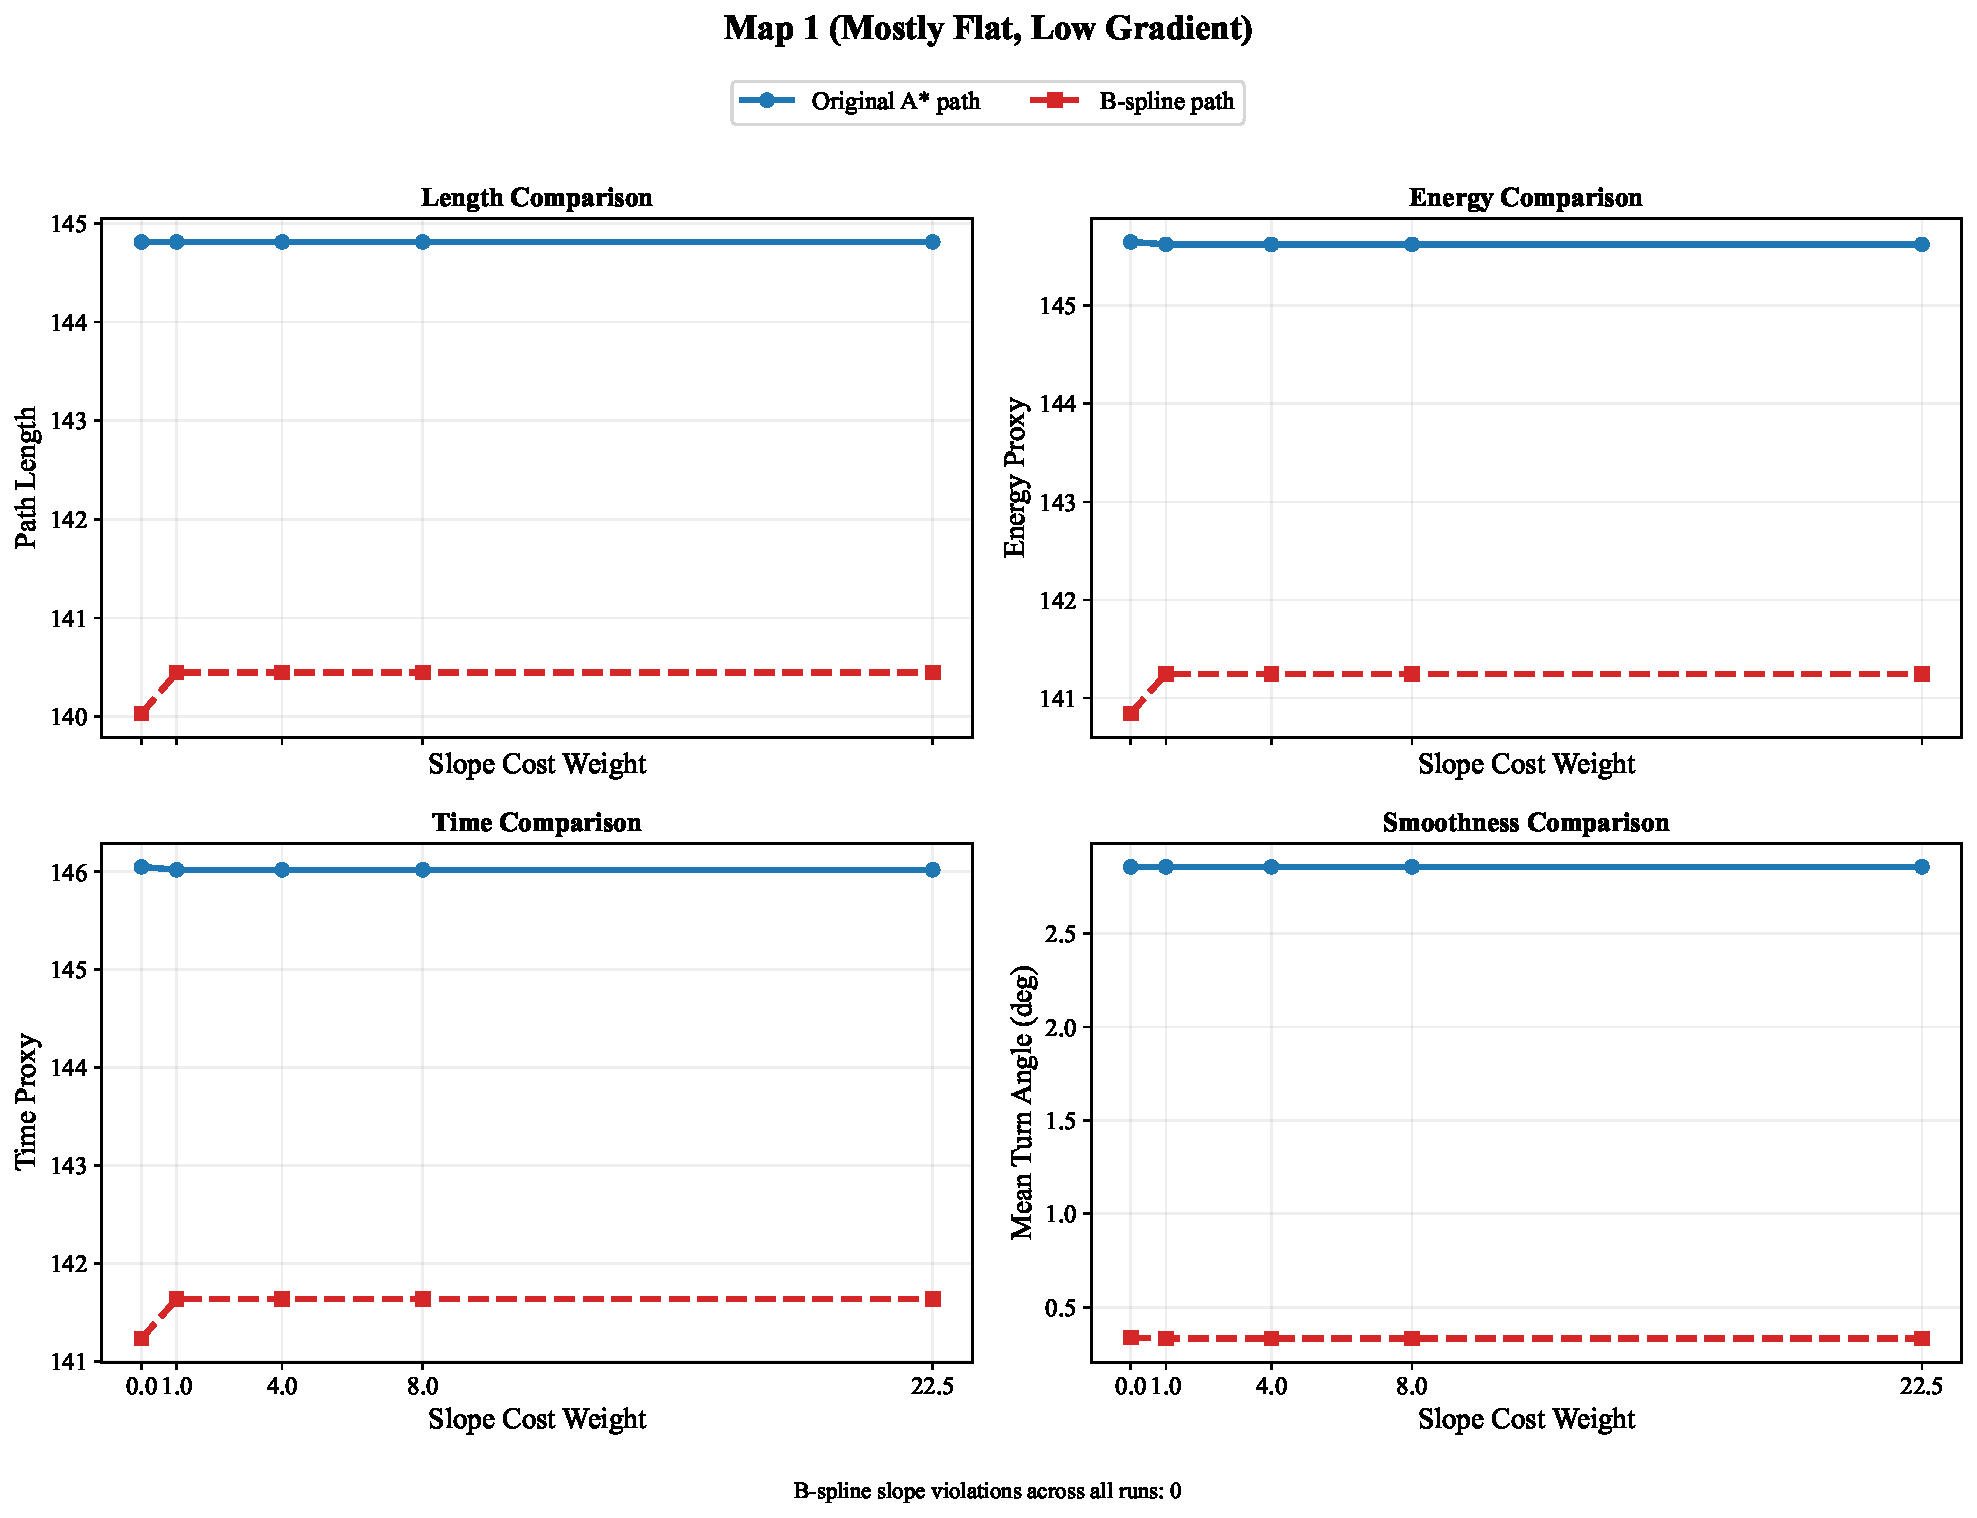
\includegraphics[width=0.48\textwidth]{figures/map1_flat_bspline.pdf}}{\fbox{\parbox{0.46\textwidth}{\centering Missing map 1 B-spline figure}}}
\hfill
\IfFileExists{figures/map2_medium_bspline.pdf}{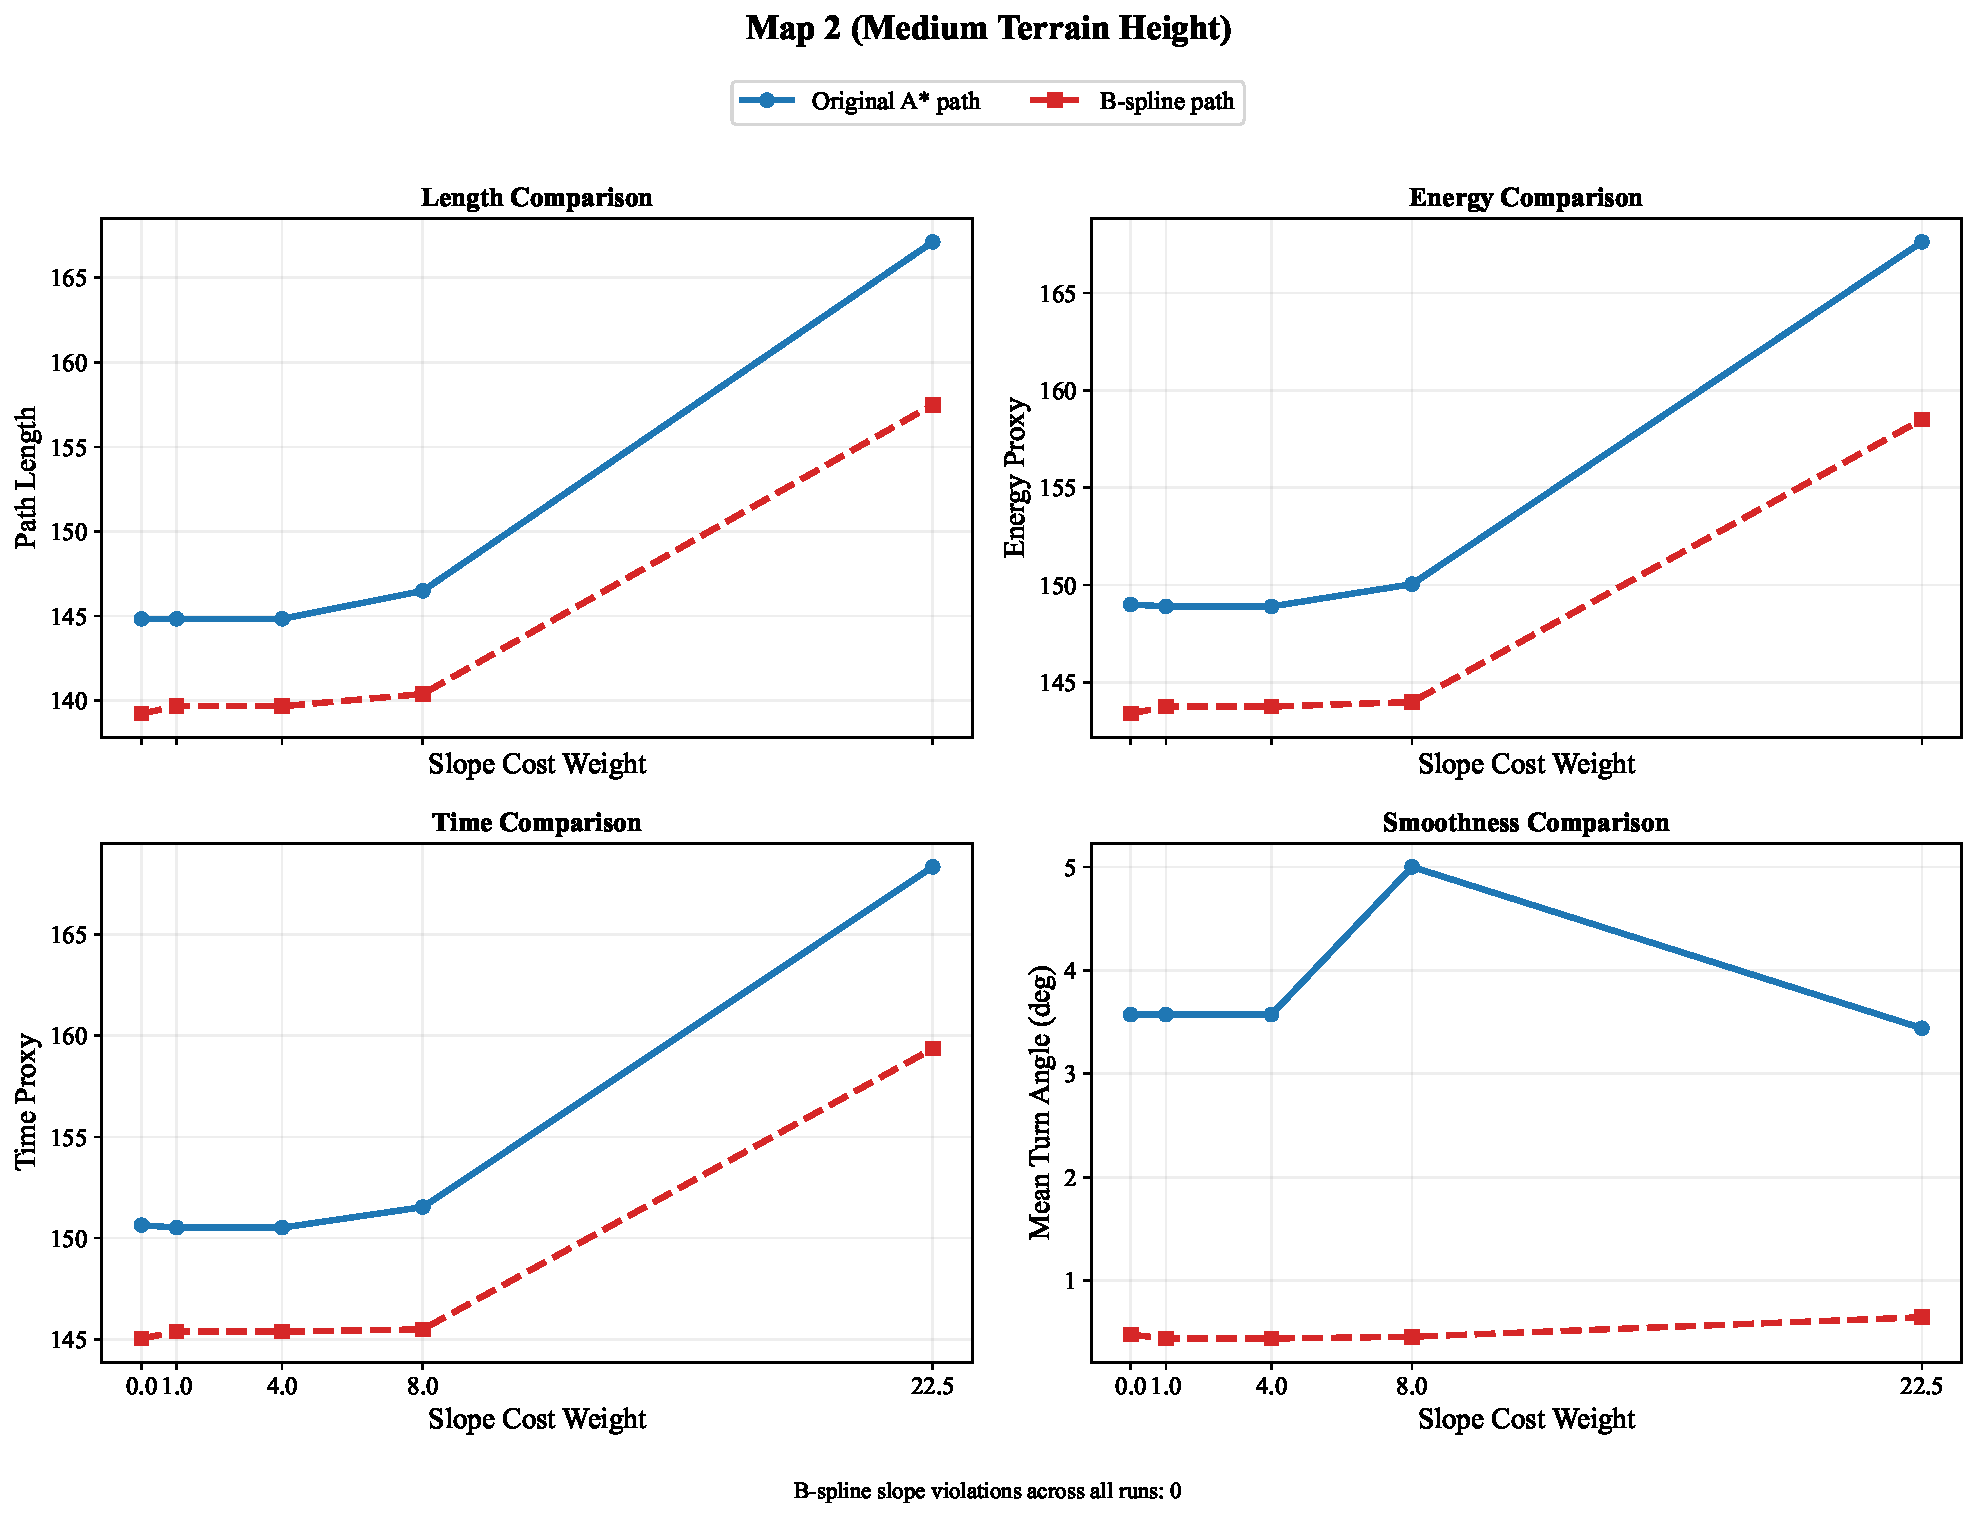
\includegraphics[width=0.48\textwidth]{figures/map2_medium_bspline.pdf}}{\fbox{\parbox{0.46\textwidth}{\centering Missing map 2 B-spline figure}}}

\vspace{0.6em}
\IfFileExists{figures/map3_high_bspline.pdf}{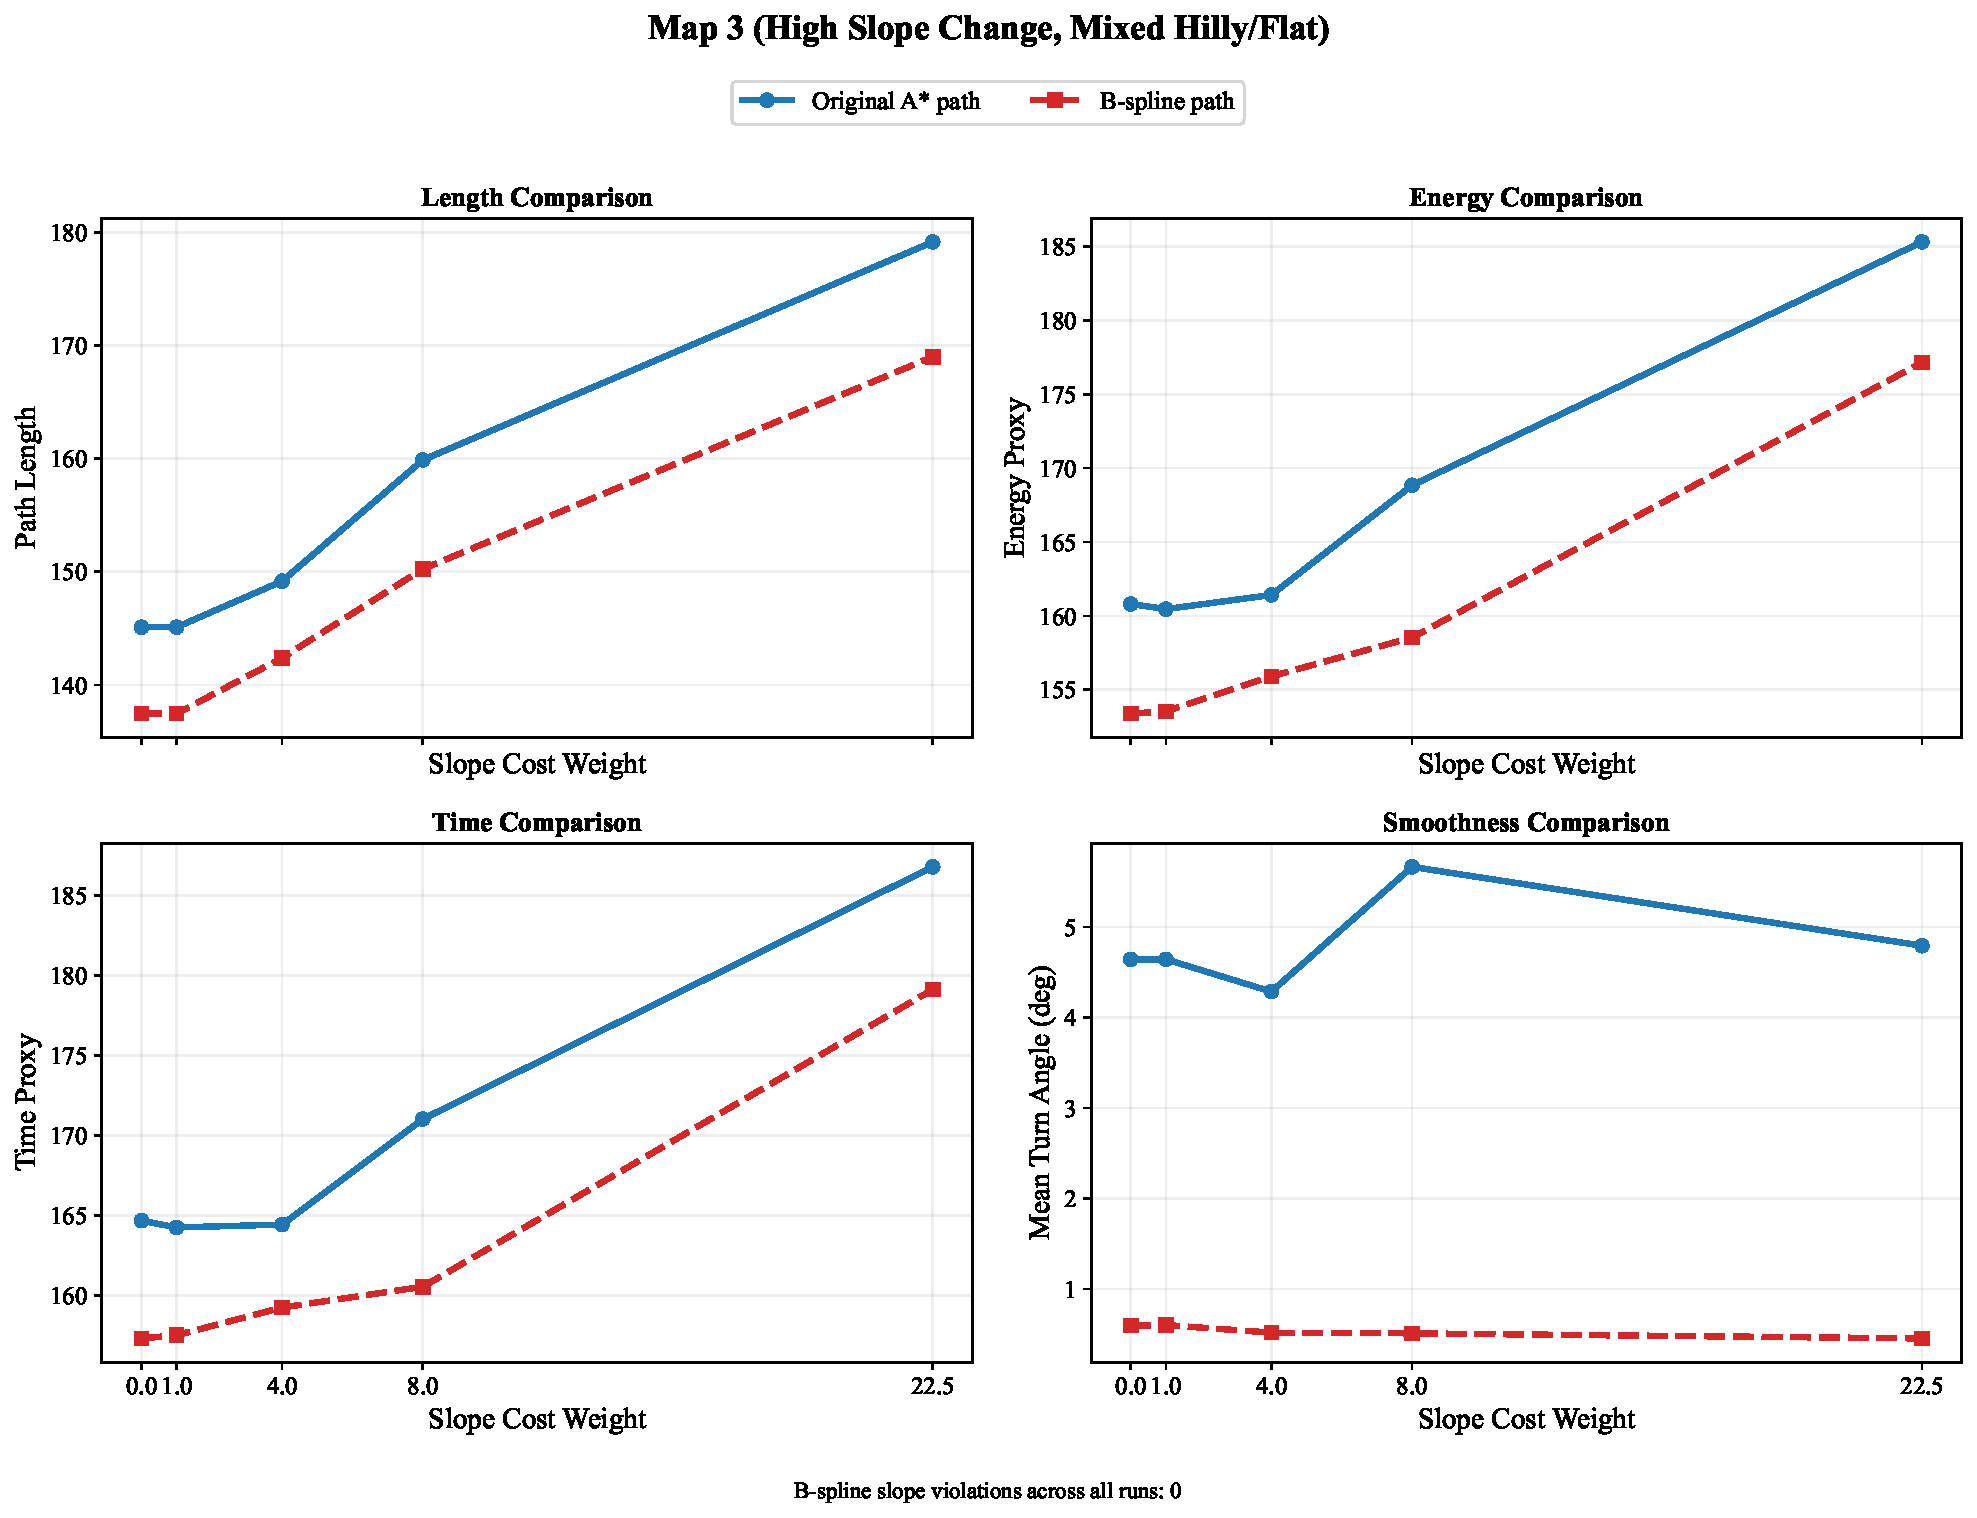
\includegraphics[width=0.62\textwidth]{figures/map3_high_bspline.pdf}}{\fbox{\parbox{0.60\textwidth}{\centering Missing map 3 B-spline figure}}}
\caption{Cross-map comparison of the original A* path and the B-spline-refined path. The dominant qualitative improvement is the significant reduction in mean turn angle, while the total path length and travel-time proxy simultaneously decrease modestly across all terrain profiles.}
\label{fig:cross_map_bspline_metrics}
\end{figure*}

These findings substantiate the assertion that the B-spline formulation serves as significantly more than a purely aesthetic visual enhancement. The refinement yields quantifiable, mathematically robust improvements in geometric regularity alongside secondary enhancements in efficiency-related proxies. Importantly, the sampled validation results show absolutely no evidence of post-smoothing slope infeasibility, verifying the safety parameters of the proposed pipeline.

\section{Threats to Validity and Future Work}
While the preliminary results are highly promising, several threats to validity remain within the current scope of the research. Firstly, the benchmark terrain maps are synthetic and deterministic; therefore, the reported behavioral trends may not perfectly capture the complex, noisy irregularities characteristic of sensor-derived agricultural field terrain. Secondly, the ECP and TTP indices function as surrogate mathematical measures rather than complete terramechanics or actuator load models; consequently, the absolute calculated values should be rigorously interpreted as comparative indicators rather than field-calibrated engineering predictions. Thirdly, the B-spline safety validation relies upon sampled slope, boundary, and vegetation checks rather than exhaustive dynamic simulation. Finally, the employed 2.5D topological representation is highly appropriate for ground-surface ground navigation but fundamentally lacks the capacity to encode structural overhangs or complex multi-layer geometry that necessitates full volumetric reasoning. 

These identified limitations do not detract from the preliminary success of the planner but actively motivate future research efforts. Subsequent stages of this thesis will focus on the integration of realistic deformable-terrain interaction models, online perception uncertainty propagation, and comprehensive physical field validation protocols.
